%!TEX root = ../thesis.tex

\chapter{Bilder}

Lorem ipsum dolor sit amet, consetetur sadipscing elitr, sed diam nonumy eirmod tempor invidunt 
\section{Ein Bild ganz breit} 
Verweis auf das Beispielbild \ref{fig:zuul}

\begin{figure}[htbp]
 \centering
 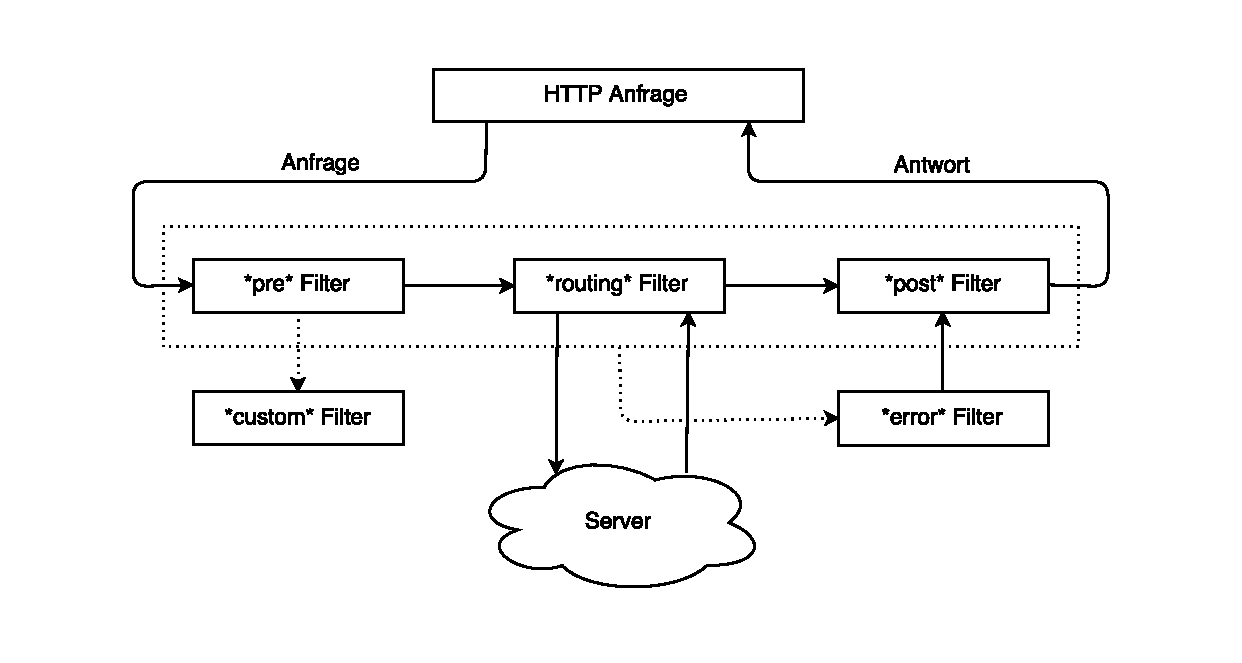
\includegraphics[width=\linewidth]{kapitel3/bilder/beispielbild}
 \caption{Beispielbild}
 \label{fig:zuul}
\end{figure}


\section{Zwei Bilder nebeneinander} 


\begin{figure}
\subfigure[Antwortzeiten]{\label{fig:antwortzeit}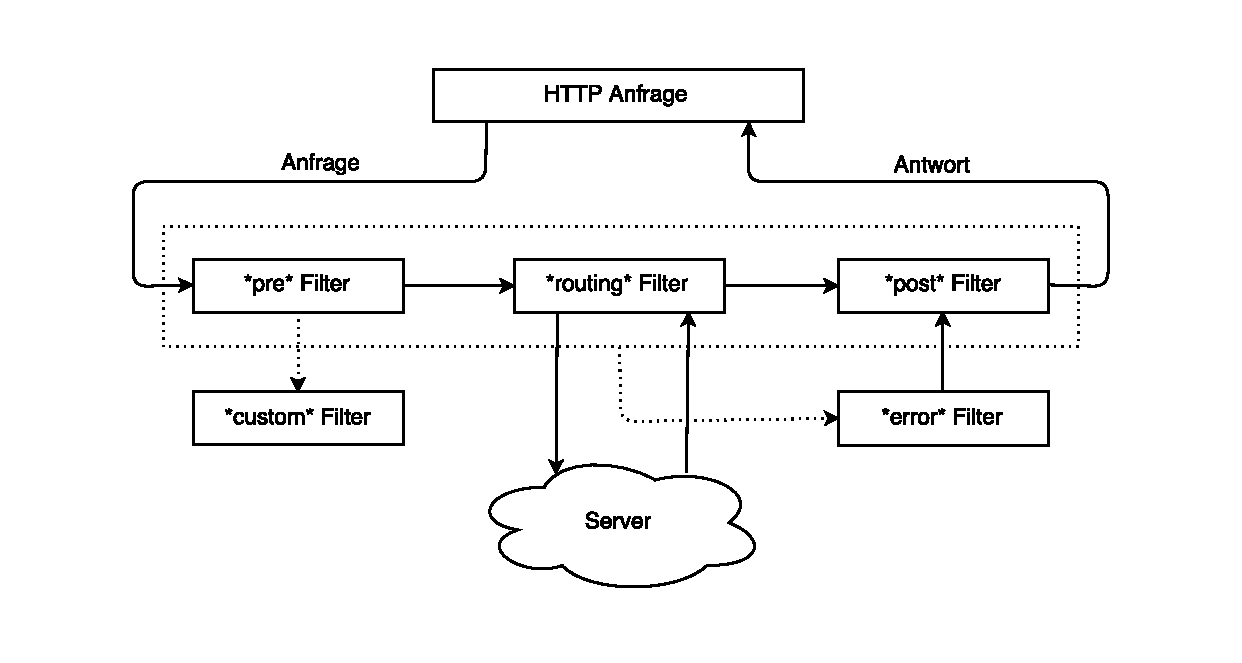
\includegraphics[width=0.50\textwidth]{kapitel3/bilder/beispielbild}}\hfill
\subfigure[prozentualer Anteil an fehlerhaften Anfragen]{\label{fig:fehler}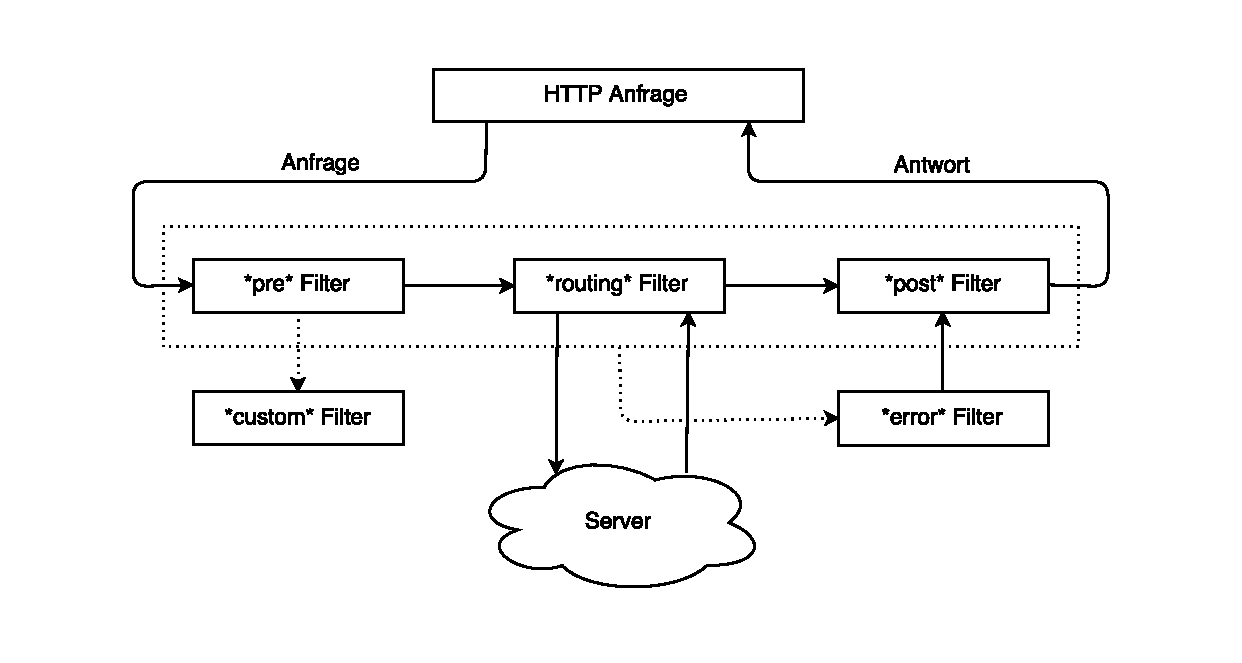
\includegraphics[width=0.50\textwidth]{kapitel3/bilder/beispielbild}}
\caption{Lasttest Szenarien}
\end{figure}

\newpage
\section{Bild mit Quellenangabe in der Fusszeile}

\begin{figure}[h]
	\centering
	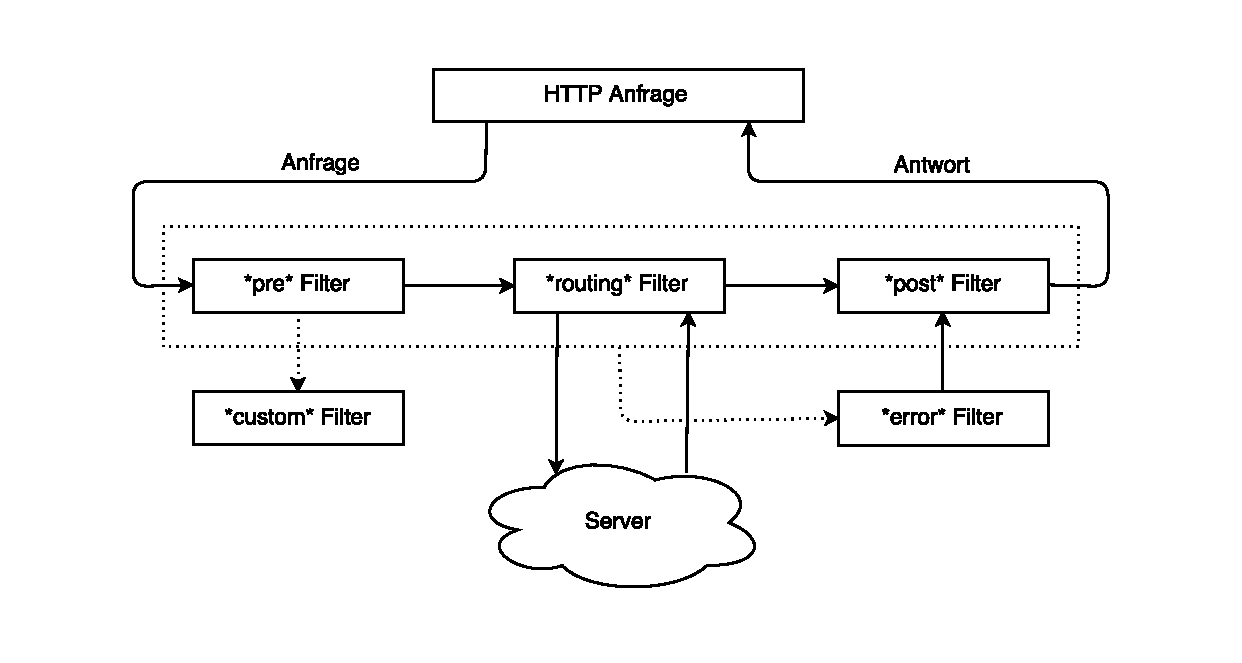
\includegraphics[width=\linewidth]{kapitel3/bilder/beispielbild}
	\caption[Beispielbild mit Qellenangabe in der Fusszeile]{Beispielbild mit Qellenangabe in der Fusszeile\protect\footnotemark}
\end{figure}
\footnotetext{Quelle: https://foo.bar/beispielbild.jpg}